
%%%%%%%%%%%%%%%%%%%%
%%% INTRODUCTION %%%
%%%%%%%%%%%%%%%%%%%%

%PROBLEM : WHICH INTERACTION TECHNIQUES TO USE WHEN DEVELOPING FOR UI REPLICATION BETWEEN A SMARTPHONE AND A TABLETOP?
%
%SOLUTION : THE PROTOTYPE, SUPPORTED BY BOTH STUDIES

\chapter{Introduction}
\label{introduction}

\begin{figure}[b!]
  \centering
    \includegraphics[width=0.6\textwidth]{images/tide3P}
  \caption{People viewing information on a smartphone.}
  \label{tide}
\end{figure}

\section{Background and motivation}

Modern smartphones are able to support most users' daily computing tasks.
They fit in a pocket, which makes them ultra mobile, and they offer good storage capacities as well as all-around connectivity.
This tendency implies that users have access to personal data and applications at all times.
Smartphones give rise to a new type of computer interaction which is unplanned, spontaneous, on-the-go.
They bring computing to situations where laptops don't fit, such as standing in a crowded train, or walking in the street.
Furthermore, they make it possible to get the most out of unforeseen opportunities, and in particular, they seem to be the ideal tool to support these chance meetings that suddenly turn into constructive collaboration.
However, the size of the device can be a limitation to this form of improvised computer interaction, especially in situations with simultaneous users. 
\\\\
Tabletop computers, on the other hand, are ideal in social contexts.
They bring computing to a very common piece of furniture, the table.
As such, they present a horizontal interactive surface around which multiple users can regroup, to share a common experience, or to conduct parallel activities.
They have been used extensively in museums and galleries, as documented by \cite{Geller:2006:exhibits}, who notes that tabletops encourage a collaborative atmosphere, and that they provide a tactile experience that reaches even the less computer literate.
Tabletops provide a touch-based experience that is fundamentally different from the traditional desktop metaphor.
A number of HCI studies show that this experience is a more natural one for the non-technical user, because it removes the mouse-and-keyboard abstraction layer and generates a more direct interaction.

\begin{figure}[htb]
  \centering
    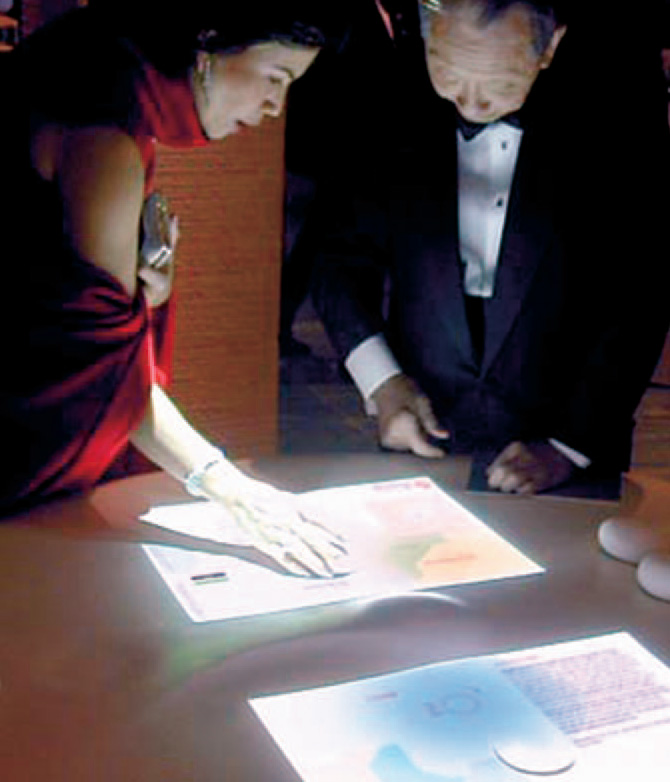
\includegraphics[width=0.4\textwidth]{images/visitors}
  \caption{People using an interactive tabletop\\exhibit at the Asia Society Museum.}
  \label{visitors}
\end{figure}

The first interactive tabletop displays were designed for individual use.
Systems such as the DigitalDesk \citep{Wellner:1993:digitaldesk} aimed at incarnating the desktop metaphor of the personal computer to the common office desk.
But tabletops have a huge potential for collaboration.
In following years, a research branch emerged that focused on \emph{smart rooms}: spaces equipped with various cutting-edge computing devices that can interoperate, to support collaborative work for multiple users.
Tabletops are an essential element of smart rooms, as shown with the InteracTable \citep{Streitz:1999:iland} and the iTable \citep{Johanson:2002:iroom}.

With the emergence of commercial items such as the Microsoft Surface \citeyearpar{ms}, tabletops are gradually appearing in public environments such as museums, meeting rooms, public lobbies, bars, restaurants, etc.
They are an ideal platform for spontaneous use and multi-user interactions, and they provide a touch-based experience that is similar than the one on most smartphones, making them easily accessible to the pubic.\\
\linebreak
%%% TECHNICAL REVIEW %%%%
%were based on overhead projected output and overhead camera-based input.
%In recent years, however, interactive displays are being commercialized, that are typically based either on computer vision or capacitance.
%
%Capacitive screens are present on the mass market since the iPhone \citep{iphone}, but are now being produced in larger sizes \citep{displax}, \citep{3m}.
%They function by sensing the electrical charge that is produced when a finger interacts with the screen's electrical field.
%This allow for a very precise touch detection, but a drawback is that it does not work with gloved fingers, digital pens or any other objects.
%
%Computer vision can be used in various ways.
%The first Microsoft Surface \citep{ms} as well as the MultiTaction displays \citep{multitouch} function with cameras that detect reflected infrared backlight from objects that are in contact with the screen.
%The main advantage of such solutions is that they can detect not only fingers, but also visual markers and other objects.
%Microsoft has perfected this technology in the latest Surface with PixelSense \citep{pixelsense}, where the individual pixels can detect what touches the screen, thus removing the need for cameras.
%PQ Labs \citep{pq} produces side vision overlays that can provide multi-touch detection to any type of screen, though without the possibility for object detection.

State-of-the-art smartphones boast screen resolutions up to 1280 by 720 pixels, that exceed the naked eye's ability to distinguish separate pixels.
%This implies beautiful graphics with profound and rich colors.
However, a smartphone screen is too small to provide a satisfying user experience in the presence of multiple users, and when viewing dense content such as text or high-quality images.
Screen sizes for ultra mobile devices go only up to 5 inches.
Reading a text, consulting a map and viewing images are examples of situations in which small displays present limitations.

An example of graphically dense content is a text of more than a few paragraphs.
The default view of an online blog or a pdf document on a smartphone is too small for a user to be able to discern single words.
Depending on one's eyesight, it usually takes 2 to 4 zooming gestures to enlarge the text to a size that is conveniently readable.
At this point, the user generally tilts the phone to a landscape orientation, to give the paragraphs a more natural length.
There is only space for 5 to 10 lines of text on the screen, which implies that the user uses successive pan gestures to update the content as s/he reads.
Compared to the casual experience of reading a newspaper article or a book, this seems like a lot of trouble.

Maps are also graphically dense.
They present a lot of different informations, such as topography, street names and sights, on limited space.
To be able to read a street name on a smartphone maps application, the user needs to zoom in on the relevant part of the map.
The result is that the user can only view a very limited area.
To be able to relate this area to, for example, his/her own location, the user must use a combination of pan and zoom out gestures that can be cumbersome.
In certain cases, the area of interest is simply too vast to be viewed on a smartphone screen.

Modern smartphones play the role of point-and-shoot cameras, due to the fact that we carry them with us at all times, and that they take pictures of high quality.
However, image viewing on a handheld device presents serious limitations.
Beside the fact that the screen is too small to do pictures justice, it makes showing them to someone else a frustrating experience.
Ideally, showing pictures to a friend implies both persons looking at the pictures together, to allow for commenting.
This is hardly possible with a smartphone.
A typical scenario is that the user finds a picture that he wants to show, then hands his phone to the friend, then the friend hands the phone back to the user, who chooses the next picture, and so on.
This process is cumbersome, and another example of the need for smartphones to be able to integrate with larger displays such as tabletops.

In the above mentioned cases, the smartphone provides all the necessary resources, with the exception of a large enough display.
This work focuses on these situations in which the smartphone experience would benefit from additional screen space.
\\
\linebreak
%It does so by suggesting a \emph{device composition} approach, that integrates smartphones and tabletops.
%Tabletops are a solution to this problem for several reasons.
%They provide the needed display space, and a touch-based interaction that comes naturally to the typical smartphone user.
%Moreover, they are designed for collocated collaboration, which brings an interesting new dimension to the scenarios discussed above.
%Examples of the possibilities include consulting a map to show a location to a friend, reading and editing a document with a colleague, playing a multiplayer game, or viewing and sharing pictures between smartphones.
A way to address this challenge is by using \emph{device composition}, a research approach that can be traced back to the work on smart space technologies and systems such as Augmented Surfaces \citep{Rekimoto:1999:augmentedsurfaces}, \mbox{i-LAND} \citep{Streitz:1999:iland} and the Interactive Workspaces \citep{Johanson:2002:iroom}.
Smart rooms were designed as closed computing environments, so recent efforts have been invested in developing for a more ad-hoc type of device composition, with projects such as Obje \citep{Edwards:2009:obje}, Platform Composition \citep{Pering:2009:platformcomp} and CompUTE \citep{Bardram:2010:compute}.

Tabletops are a central device in the aforementioned smart rooms, and a recurring element within device composition.
They are an ideal platform for collocated collaboration, as was shown with systems such as the MemTable \citep{Hunter:2011:memtable} and SketchTop \citep{Clifton:2010:sketchtop}, that are designed to support the work of technical users.
In recent years, however, tabletops are appearing in public spaces, aiming at engaging common users in a more casual form of interaction.
\\
\linebreak
Within this context, designing for device composition between smartphones and tabletops implies addressing three fundamental challenges.

The first one is the pairing procedure responsible for device discovery and connection.
Pairing between unknown devices has been solved in many different ways.
An example that is particularly relevant to this work is the BlueTable \citep{Wilson:2007:bluetable}, an interactive surface that uses Bluetooth to discover and connect to a mobile phone, but improves this process by using computer vision to locate the phone on the table, and verify its identity via the phone blinking an infrared signal.

The second challenge is how to distribute the UI of the smartphone to the tabletop.
There exists various stable technologies to choose from, but recent research works have chosen to build frameworks from scratch, to allow a more flexible distribution and sharing of user interfaces between multiple types of devices.
An example of such an approach is XICE (eXtending Interactive Computing Everywhere) \citep{Arthur:2011:xice}, a programming framework that is destined to support a new form of nomadic experience, where users can annex various display servers with their mobile personal devices.

The last challenge is to design a user interaction that suits the purpose of the system.
Different interaction metaphors have been used to extend the UI of smartphones to larger display surfaces, including streaming, replication, expansion, projection and adaptation.
In their recent work on Virtual Projection (VP), \cite{Baur:2012:virtualprojection} built a system where a smartphone can be used to seemingly project its UI onto an available computer display.

%Device composition started with SMART ROOMS, and composing various devices, which we want to do in this case.
%But smart rooms were designed as closed environments.
%
%We would like AD-HOC, spontaneous device composition.
%That was addressed by projects like Obje, CompUTE, Platform Composition.
%
%we are interested in mobile to TABLETOP
%- studies on collaboration (but closed environments and technical users)
%- studies on tangible interaction
%
%tabletops emerge in public spaces > non technical users > we focus on standard hardware
%
%we must solve 3 challenges: pairing, UI distributing, user interaction
%
%To combine SP and TT, we need to pair them, which can be done
%with networked protocols or bluetooth
%(but that requires explicit input from user, or CPU/battery intensive continuous sniffing
%SO we use a trigger, that can be:)
%detecting synchronous events
%entering a key into display
%with RFID
%with computer vision to detect
%
%we do it with computer vision detection and networked protocol (Bonjour)
%
%we need a technology to do UI distribution:
%distr data
%distr code
%
%best to distr graphics:
%(we choose VNC in spite of drawbacks > why?)
%
%we need a user interaction
%
%FINISH with how we do differently!

\section{Problem statement}

This thesis addresses the problem of using \emph{consistent} design to build a composite device between a smartphone and a tabletop computer, that allows for \emph{spontaneous interaction}.
\\
\linebreak
It does so by answering the following research questions:
\begin{itemize}
\item What are the requirements for such a system?
\item Which interaction techniques are best suited to this type of system?
\item Can this system be made to run on standard hardware and integrate different smartphone types?
\end{itemize}

\section{Research methods}

To solve the problem at hand, the following research methods were used.
\\
\linebreak
To place the present work within its research context, 
a comprehensive literary review was made of the prior work related to device composition and surface computing.
In particular, the following aspects of device composition were investigated: main approaches, tabletop systems and applications, pairing, UI distribution, user interaction.
The resulting study is presented in Chapter~\ref{relatedwork}.

Following a user-centered approach, a solution design was completed.
The process was divided into to the following tasks.
The application's context of use was analyzed with the support of scenarios and storyboards, which lead to the definition of solution requirements.
A series of design options were generated from the study of existing approaches to software design for surface computing.
With the support of a study based on low-fidelity prototypes and the involvement of potential users, a final design was produced.
The design process is reported in Chapter~\ref{design}

In order to demonstrate the feasibility of the suggested solution, a proof of concept was realized, in the form of an application prototype implemented on the Microsoft Surface tabletop computer, an iPhone 4 and a HTC Legend phone.
The implementation was focused on the user interaction, in the aim of showing that consistent design can lead to an easy user experience.
The system is described in Chapter~\ref{system}.

%Third-party applications are used on the smartphones, that requires rooting the devices.
%On the tabletop computer, the application is programmed within the .NET framework,  using specifically WPF (Windows Presentation Foundations) and the Presentation layer of the Microsoft Surface API 1.0.

An evaluation of the design was conducted by way of a usability study, that involved the following steps.
The focus of the evaluation was identified, in terms of specific aspects of the system, and the evaluation methods were selected.
A user experiment was designed, that involved a discovery phase, cooperative evaluation, a semi-controlled test and a questionnaire.
Participants were recruited, and the experiment was carried out.
Evaluation data was gathered via online forms as well as application logging.
The resulting data was processed, analyzed, and the evaluation results were derived.
The evaluation process and results are presented in reported in Chapter~\ref{evaluation}.

\section{Contributions}

This work consists of the design, implementation and evaluation of a composite device that integrates smartphones to the Microsoft Surface.
There are three major contributions.

\begin{enumerate}

\item The user-centered design process shows that it is feasible to design a system that is immediately accessible to all types of users, and that the user interaction plays an essential role in the design of an intuitive device.
To support the process of selecting the most intuitive interaction techniques, this work introduces two design principles: \emph{consistency} and \emph{physicality}.
The consistency of the design refers to the selection of interaction techniques that users already know from any type of prior experience.
The physicality of the design implies taking into consideration the form factor of the devices, to identify interaction techniques that are natural to the user.
%The tabletop interaction should be consistent with the smartphone interaction, reacting whenever possible as the user would expect a smartphone to.
%Well-known interaction techniques, such as the double tap, are easy for the user to discover, and can therefore be used accordingly.
%The physical form of the devices has implications on the user's expectations, that the interaction should be consistent with.
%Some implications can be translated to the design, such as the common expectation that moving a document off a table takes the focus away from it.

\item The implementation of the proof-of-concept application called \emph{TIDE (Tabletop Interactive Display Extension)} shows that it is feasible to implement a system on the Microsoft Surface (first generation) that allows users to integrate any type of smartphone to the tabletop by way of UI replication.
%It shows that the pairing procedure can be made quick and easy by using camera-based object detection and wireless connectivity.
%The display of the smartphone is replicated to the tabletop, and is referred to as the \emph{remote UI}, allowing the user to interact with his phone indirectly.
%The remote UI is contained in an application window that is referred to as the \emph{surface UI}, whose role is to allow for the manipulation of the remote UI on the tabletop display.
%The UI replication is based on the VNC protocol \citep{Richardson:1998:vnc}.
%Currently supported devices are iOS and Android smartphones, but TIDE can be extended to support other devices.

\item The final contribution is the evaluation of the application design.
It shows that consistency and physicality allow the design of a device that is easy to use for all types of users.
Furthermore, it shows that it is a good idea to implement several interaction techniques for a same feature, in order to reach users with different background.
Finally, the evaluation confirms that there is a need for a system that allows users to extend their smartphone screen space to a larger display.

\end{enumerate}

%\section{Thesis overview}
%
%Chapter~\ref{relatedwork} presents a literary review of the research that constitutes the background to this work, and the theoretical work on which the design approach is based.\\
%Chapter~\ref{design} describes the process that lead to the design of the TIDE prototype.\\
%The system itself is presented in Chapter~\ref{system}, and its evaluation by way of a usability study in Chapter~\ref{evaluation}.\\
%Chapter~\ref{discussion} is a discussion that addresses the results and lessons learned throughout this process, and brings suggestions for future work.\\
%Chapter~\ref{conclusion} concludes the report.

% solution : using tabletops as UI peripherals
%%%%%%%%%%%%%%%%%%%%%%%%%%%%%%%%%%%%%%
%The specificity of tabletops raises the question of how to interact with them on an everyday basis.
%Recent development initiatives tend to answer this question by regarding tabletops as yet another computational platform, requiring its own software.
%With this project, we explore a different approach to integrating tabletops in our environment, namely by using them only as UI peripheral, providing touch-based input and graphical output to the devices that we already have.
%Exploring this path is supported by three important factors.
%First, most users already own computing devices, such as laptops or smart phones, with tailor-made applications and local storage, and might be less prone to use an additional device if it requires management (updates, backups, synchronizations, etc) and the purchase of applications.
%Second, tabletops are embedded in the environment and as such can be expected to be shared devices.
%Using them as simple graphic peripheral would allow to avoid the traditional desktop/laptop issues related to user profiles, privacy and data integrity.
%Finally, as embedded devices, it is reasonable to expect tabletops to have good networking capabilities.

% device composition
%%%%%%%%%%%%%%%%%%%%%%%%%%%%%%%%%%%%%%
%Device composition focuses on getting the most out of various computing entities, by making them work together and function as one, as seen in \cite{Bardram:2010:compute}.
%This project explores device composition for UI integration between tabletops and mobile devices, focusing on seamless user experience and implicit human computer interaction as defined by Schmidt in \cite{Schmidt:2000:implicit}.

% UI integration metaphors
%%%%%%%%%%%%%%%%%%%%%%%%%%%%%%%%%%%%%%
%UI integration can happen in several different ways:
%\begin{itemize}
%\item{\emph{UI transfer} (mirror): the tabletop `takes over' and displays the UI of the connected device.}
%\item{\emph{Dual view}: the tabletop display becomes secondary screen space for the connected device.}
%\item{\emph{UI nesting}: the connected device is physically located on the tabletop, and its UI is extended to the additional screen space around it.}
%\end{itemize}

% challenges
%%%%%%%%%%%%%%%%%%%%%%%%%%%%%%%%%%%%%%
%Following is an open list of problems that we will address in order to achieve device composition by means of implicit interaction.
%\begin{enumerate}
%\item{\emph{Setup}: How is a device enabled for integrating with a tabletop?
%The setup should be simple, to be performed only once by non-technical users.
%An initial survey of possible solutions points towards the use of tagging mechanisms and/or camera-based object recognition.}
%\item{\emph{Discovery}: How do the tabletop and the device discover and communicate with each other?
%How do we solve the issues of discovery, handshake, network connectivity, and encryption mechanisms to ensure privacy?}
%\item{\emph{UI transfer}: Given the computational constraints of mobile devices, how can the UI transfer be efficiently implemented so as to support native applications and guarantee a seamless user experience?}
%\item{\emph{Input}: How can the users interact with their applications on the tabletop (touch and other peripherals)?}
%\item{\emph{Interaction Design}: What means of interaction are best-fitted for the tabletop-based systems that we propose to develop?
%How can we best adapt to public/private uses and single/multiple users?
%How can we take advantage of the larger interaction surface?}
%\end{enumerate}

